\documentclass{article}
\usepackage[utf8]{inputenc}
%\pagenumbering{Roman}
\usepackage{ragged2e}
\usepackage{graphicx}
\usepackage{wrapfig}
\usepackage[table,xcdraw]{xcolor}
\usepackage{hyperref}
\hypersetup{
	colorlinks=true,
	linkcolor=blue,
	filecolor=magenta,      
	urlcolor=cyan,
	pdftitle={Overleaf Example},
	pdfpagemode=FullScreen,
}

\title{\huge Interface S88 Gleisbox Raspberry Pi Manual}
\author{Guido de Hek}
\date{\today}

\setlength{\parindent}{0pt}

\begin{document}

	\maketitle
	
	\newpage
	
	%% Table of contents
	\tableofcontents
	\clearpage
	
	
	%% Introduction
	\section*{Credits}
Parts of this system have been developed by members of the model railway community. This is mainly applicable for the s88udp conversion, as well as srcpd. Many thanks and full credits to them!

\newpage

\section{Introduction}
System for controlling a marklin track using a rpi
	\newpage
	
	%%Setup of the raspberry pi
	\section{Setup of the Raspberry Pi}
Prepare an SD-card with Raspberry Pi OS. I have used the version from October 10th 2023 (64-bit) with desktop but without recommended software. My system uses a Raspberry Pi 4B. The advantage of desktop support is that a standalone system can be created by attaching an external monitor, mouse and keyboard. This creates the possibillity of implementing a very small and modular control system.\\

Refer to the \href{https://projects.raspberrypi.org/en/projects/raspberry-pi-setting-up/2}{Raspberry Pi website} for instructions. Follow the instructions to setup the raspberry pi OS. For remote control of the raspberry pi it is possible to enable SSH and/or VNC. Refer to the \href{https://projects.raspberrypi.org/en/projects/raspberry-pi-setting-up/4}{setup instructions} for more information. There is a lot of information available about the setup and realizing SSH or VNC communication on Raspberry Pi support forums.

\subsection{Install BCM2835 v1.73}
Install BCM2835-1.73 so that the pin IO on the Raspberry Pi can be used:
%% setup bmc
\begin{verbatim}
	wget http://www.airspayce.com/mikem/bcm2835/bcm2835-1.73.tar.gz 
	
	tar zxvf bcm2835-1.73.tar.gz
	
	cd bcm2835-1.73
	
	./configure
	
	make
	
	sudo make check
	
	sudo make install
\end{verbatim}

\subsection{Shutdown Button}

% https://howchoo.com/g/mwnlytk3zmm/how-to-add-a-power-button-to-your-raspberry-pi

A button can be connected to the system to simplify the process of shutting the system down. First of all, a pushbutton must be connected between GPIO3 (header pin 5) and GND (e.g. header pin 6). \\

Next, the following script must be installed:

\begin{verbatim}
	git clone https://github.com/Howchoo/pi-power-button.git
	
	./pi-power-button/script/install
\end{verbatim}

Uninstalling the script can be done via:

\begin{verbatim}
	./pi-power-button/script/uninstall
\end{verbatim}

Note: warning about pull-up resistor can be neglected.
	\newpage
	
	%%Setup of CAN-interface
	\section{Setup of CAN-interface}
t.b.d.

\subsection{Connection Scheme}
The CAN-bus shall be connected to the Gleisbox as depicted in figure~\ref{fig:mobilestation2_din10}. The pin 1 (power supply) does not have to be connected.


\begin{figure}[h!]
	\centering
	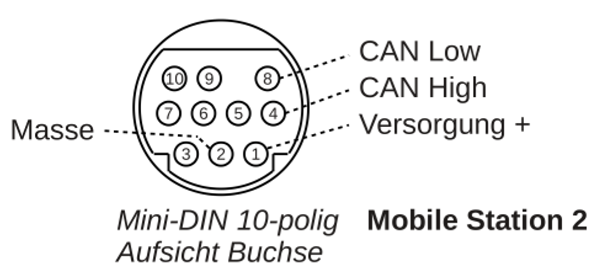
\includegraphics[width=1.00\linewidth]{../figures/mobilestation2_din10.png}
	\caption{Pinout canbus.}
	\label{fig:mobilestation2_din10}
\end{figure}

\subsection{Oscillator Settings}



\begin{figure}[h!]
	\centering
	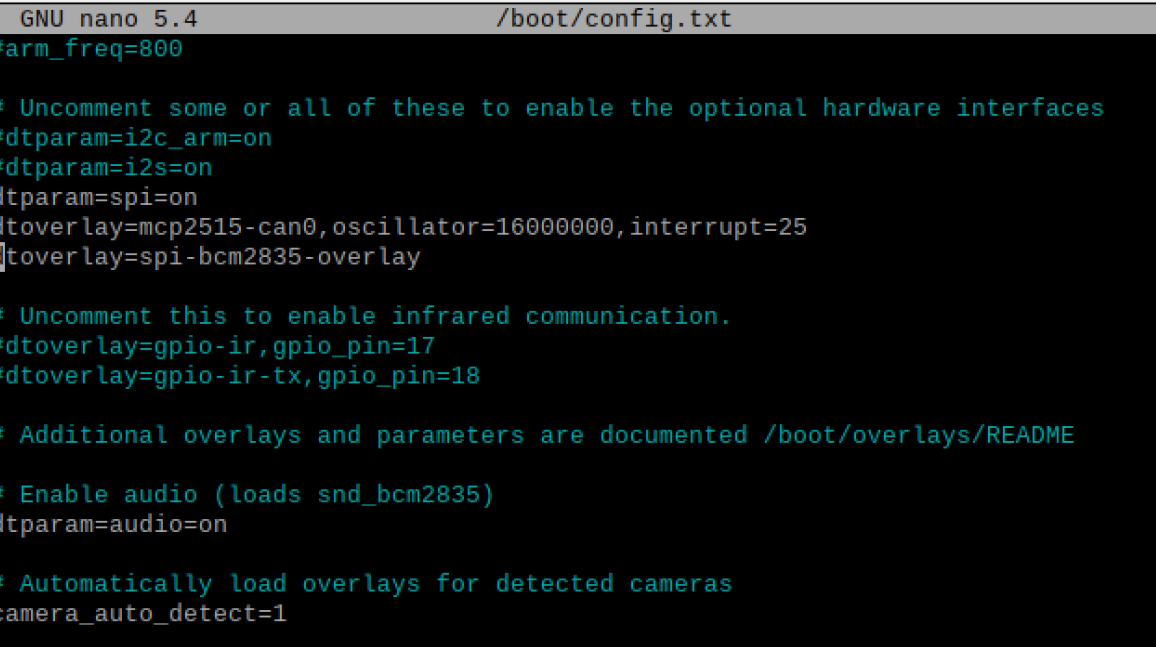
\includegraphics[width=1.00\linewidth]{../figures/oscillatorSettingsConfigTxt.png}
	\caption{Pi Oscillator settings.}
	\label{fig:oscillatorSettingsConfigTxt}
\end{figure}

sudo ip link set can0 up type can bitrate 250000 restart-ms 100


\subsection{Rocrail Server Settings}



\begin{figure}[h!]
	\centering
	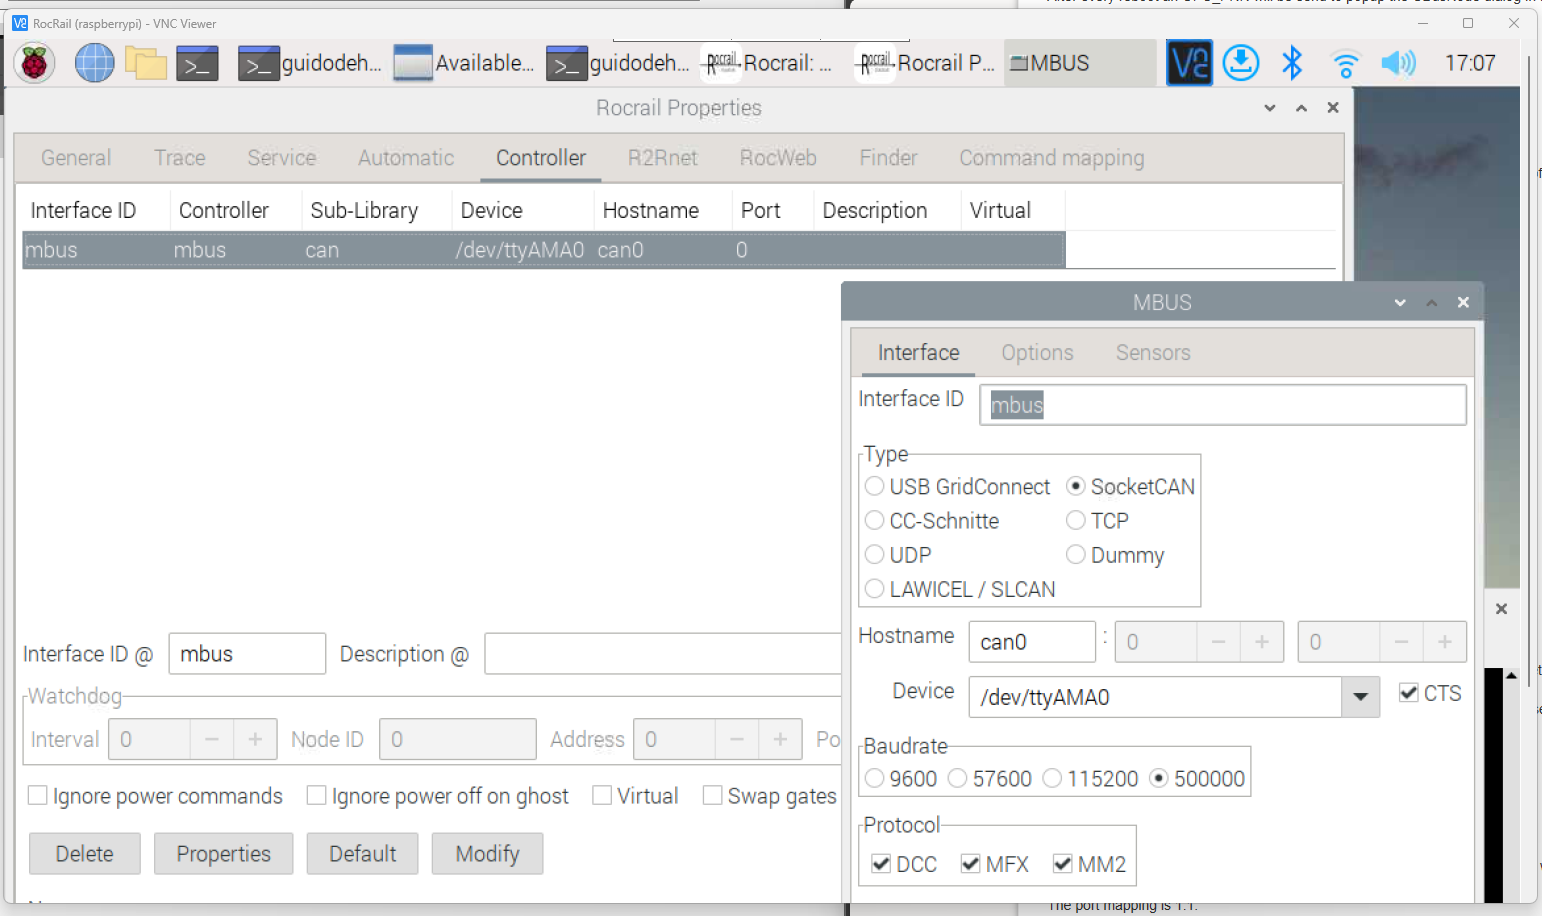
\includegraphics[width=1.00\linewidth]{../figures/rocrailServerSettings.png}
	\caption{rocrailServerSettings.}
	\label{fig:rocrailServerSettings}
\end{figure}



	\newpage
	
	%%Setup of S88n-interface
	\section{Setup of S88n-interface}
t.b.d.

\subsection{Connection Scheme}
	
%https://www.floodland.nl/aim/info_s88_kabels_en_1.htm


\begin{table}[]
	\caption{S88N pinout and description.}
	\label{tab:my-table}
	\begin{tabular}{|l|l|l|}
		\hline
		\rowcolor[HTML]{9B9B9B} 
		\textbf{RJ45 pin} & \textbf{Colour in UTP cable} & \textbf{S88N Description}             \\ \hline
		1                 & Orange-white                 & +5V (+12V not in this board)          \\ \hline
		2                 & Orange                       & Data                                  \\ \hline
		3                 & Green-white                  & GND                                   \\ \hline
		4                 & Blue                         & Clock                                 \\ \hline
		5                 & Blue-white                   & GND                                   \\ \hline
		6                 & Green                        & Load                                  \\ \hline
		7                 & Brown-white                  & Reset                                 \\ \hline
		8                 & Brown                        & Rail signal (not used in this design) \\ \hline
	\end{tabular}
\end{table}
	\newpage

	%%PCB description
	\section{PCB Description}


\begin{figure}[h!]
	\centering
	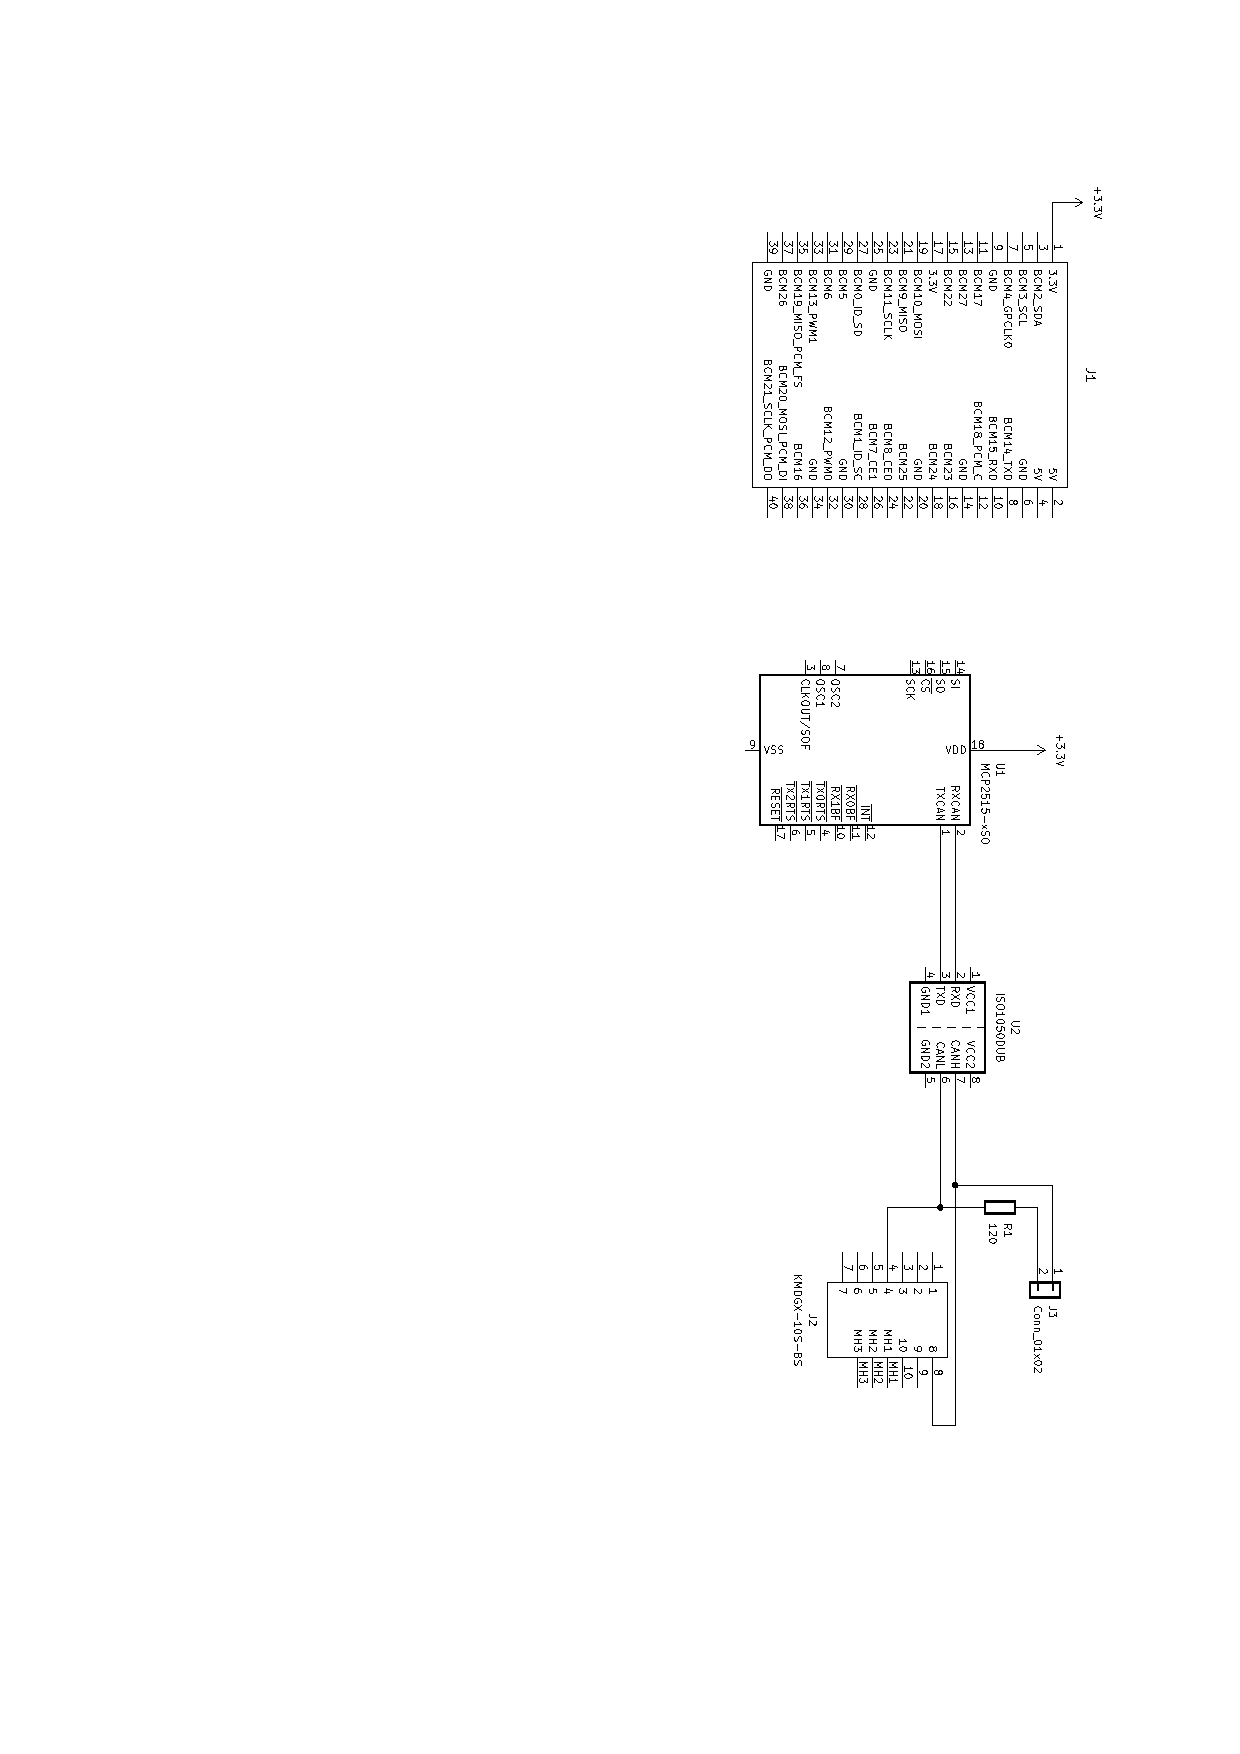
\includegraphics[width=1.00\linewidth]{../../pcb/InterfaceS88GleisboxRPi/InterfaceS88GleisboxRPi.pdf}
	\caption{Schematic of the system.}
	\label{fig:pcbschematic}
\end{figure}
	\newpage

\end{document}